\documentclass[t]{beamer}

% Load general definitions
% Preamble file - general definitions, package loading, etc.

%=================================
% Load packages
\usepackage{amssymb,amsmath}
\usepackage{graphicx}
\usepackage{url}
\usepackage{tikz}
\usetikzlibrary{mindmap,trees,arrows}
\usepackage{fancyvrb}
\usepackage[portuguese]{babel} 
\usepackage[utf8]{inputenc}
\usepackage{subfigure}
\usepackage{times}
\usepackage[T1]{fontenc}
\usepackage{cancel}
\usepackage{color}
\usepackage{listings}
\usepackage[document]{ragged2e}
\usepackage{hyperref}
\usepackage{listings}


%=================================
% Set mode
\mode<presentation>
{
	\usetheme{Madrid}
	\usecolortheme{structure}
	\useoutertheme{infolines}
	\setbeamercovered{invisible}
}

% Get rid of nav bar
\beamertemplatenavigationsymbolsempty

% Insert frame number at bottom of the page.
\usefoottemplate{\hfil\tiny{\color{black!90}\insertframenumber}} 

%=================================
% Define new commands

\newcommand\Real{{\mathbb{R}}}
%\newcommand{\vi}{\vspace{0.6\baselineskip}}
%\newcommand{\goodgap}{\hspace{\subfigtopskip}\hspace{\subfigbottomskip}}


% Equation environments
\newcommand{\beq}{\begin{equation}}
\newcommand{\eq}{\end{equation}}
\newcommand{\beqs}{\begin{equation*}}
\newcommand{\eqs}{\end{equation*}}
\newcommand{\beqn}{\begin{eqnarray}}
\newcommand{\eqn}{\end{eqnarray}}
% Bold variables
\newcommand{\mbf}[1]{\ensuremath{\mathbf{#1}}}
% Itemization
\newcommand{\bitem}{\begin{itemize}}
\newcommand{\eitem}{\end{itemize}}
\newcommand{\spitem}{\vskip 1em\item}
\newcommand{\bitems}{\begin{itemize}\item}
\newcommand{\benums}{\begin{enumerate}\item}
\newcommand{\eenum}{\end{enumerate}}
% color blocks
\newenvironment{colorblock}[2]{%
\setbeamercolor{block title}{#2}
\begin{block}{#1}}{\end{block}}
% Vertical spacing
\newcommand{\vone}{\vskip 1em}
\newcommand{\vhalf}{\vskip .5em}
% Frame environments
\newenvironment{ftst}[3][t]{%
\begin{frame}{environment=ftst,#1}
\frametitle{#2}
\framesubtitle{#3}}{\end{frame}}
\newenvironment{ftstf}[2]{
\begin{frame}[fragile,environment=ftstf]
\frametitle{#1}
\framesubtitle{#2}}{\end{frame}}
% colors
\definecolor{MyGray}{rgb}{0.5,0.5,0.5}
\definecolor{MyDBGray}{rgb}{0.1,0.1,0.4}
\definecolor{darkgreen}{rgb}{0,0.4,0}
\definecolor{black}{rgb}{0,0,0}
\def\defn#1{{\color{red} #1}}
% Footnote
\renewcommand{\thefootnote}{\alph{footnote}}
% Relaxed footnotes
\newcommand{\lfr}[1]{\let\thefootnote\relax\footnote{\tiny #1}}
% Verbatim environment - using FANCYVRB package
\DefineVerbatimEnvironment%
{rcode}{Verbatim}
{fontsize=\scriptsize}

% Verbatim environment - using LISTINGS package
%\lstnewenvironment{rcode} {\lstset{	language = R,
%									basicstyle = \scriptsize\ttfamily,
%									showspaces = false,
%									showstringspaces = false,
%									showtabs = false,
%									keywordstyle = \color{black}\bfseries,
%									commentstyle = \color{darkgreen},
%									numbers = none,
%									otherkeywords={	<-,
%													ggplot,
%													geom_boxplot,
%													facet_grid,
%													shapiro.test,
%													fligner.test,
%													glht,
%													with},
%									deletekeywords={data,
%													model,
%													residuals,
%													c,
%													axis,
%													default,
%													labels,
%													qq.text}}}%
%{}

% Specific definitions
\title[]{Tópicos Especiais em Computação I}
\subtitle[]{Caracterização dos dados}
\author[]{Patrícia Lucas\\{\footnotesize }}
\institute{Bacharelado em Sistemas de Informação \\ IFNMG  - Campus Salinas}
\date{\scriptsize Salinas\\Setembro 2021}

\begin{document}

% cover page
\setbeamertemplate{footline}{}
\begin{frame}

\begin{center}
\includegraphics[width=.15\textwidth]{}
\end{center}
  \titlepage
  \begin{tikzpicture}[remember picture,overlay]
  \node[anchor=south east,xshift=-5pt,yshift=5pt] at (current page.south east) {\tiny Versão 1.2021};
  \node[anchor=south west,yshift=0pt] at (current page.south west) {
\includegraphics[width=.25\textwidth]{Logos/salinas_horizontal_jpg.jpg}};
  \end{tikzpicture}  
\end{frame}

% Main slides
\begin{ftst}{Caracterização dos dados}{Referência}

\begin{figure}
    
\includegraphics[scale=0.35]{Figuras/slide01_11.jpg}
\end{figure}
Capítulo 2: Análise de dados.
\vone
\scriptsize
Inteligência Artificial: Uma abordagem de aprendizado de máquina. Katti Faceli...[et al.]. - Rio de Janeiro: LTC, 2011.

\end{ftst}

%=====

\begin{ftst}{Conjuntos de dados}{Análise dos dados}

\textbf{Quantos dados são gerados a cada dia?}
\vone
\item 500 milhões de tweets são enviados.

294 bilhões de e-mails são enviados.

4 petabytes de dados são criados no Facebook.

4 terabytes de dados são criados a partir de cada carro conectado.

65 bilhões de mensagens são enviadas no WhatsApp.

5 bilhões de pesquisas são feitas.
\vone
Em 2025, estima-se que 463 exabytes de dados serão criados a cada dia em todo o mundo - isso é o equivalente a 212.765.957 DVDs por dia!
\vone
\vone
\vone
\scriptsize
\href{https://www.weforum.org/agenda/2019/04/how-much-data-is-generated-each-day-cf4bddf29f/}{https://www.weforum.org/agenda/2019/04/how-much-data-is-generated-each-day-cf4bddf29f/}
\end{ftst}

%=====

\begin{ftst}{Conjuntos de dados}{Análise dos dados}

Além de serem gerados por várias fontes diferentes, esses dados também assumem formatos diferentes:
\vone
\begin{itemize}
    \item Séries temporais
    \item Imagens
    \item Vídeos
    \item grafos
    \item texto
    \item páginas web...
\end{itemize}

\vone

\centering \include{Figuras/grafo_regular}

\end{ftst}


%=====

\begin{ftst}{Natureza dos dados}{Caracterização dos dados}
\vone
\begin{figure}
    \centering
    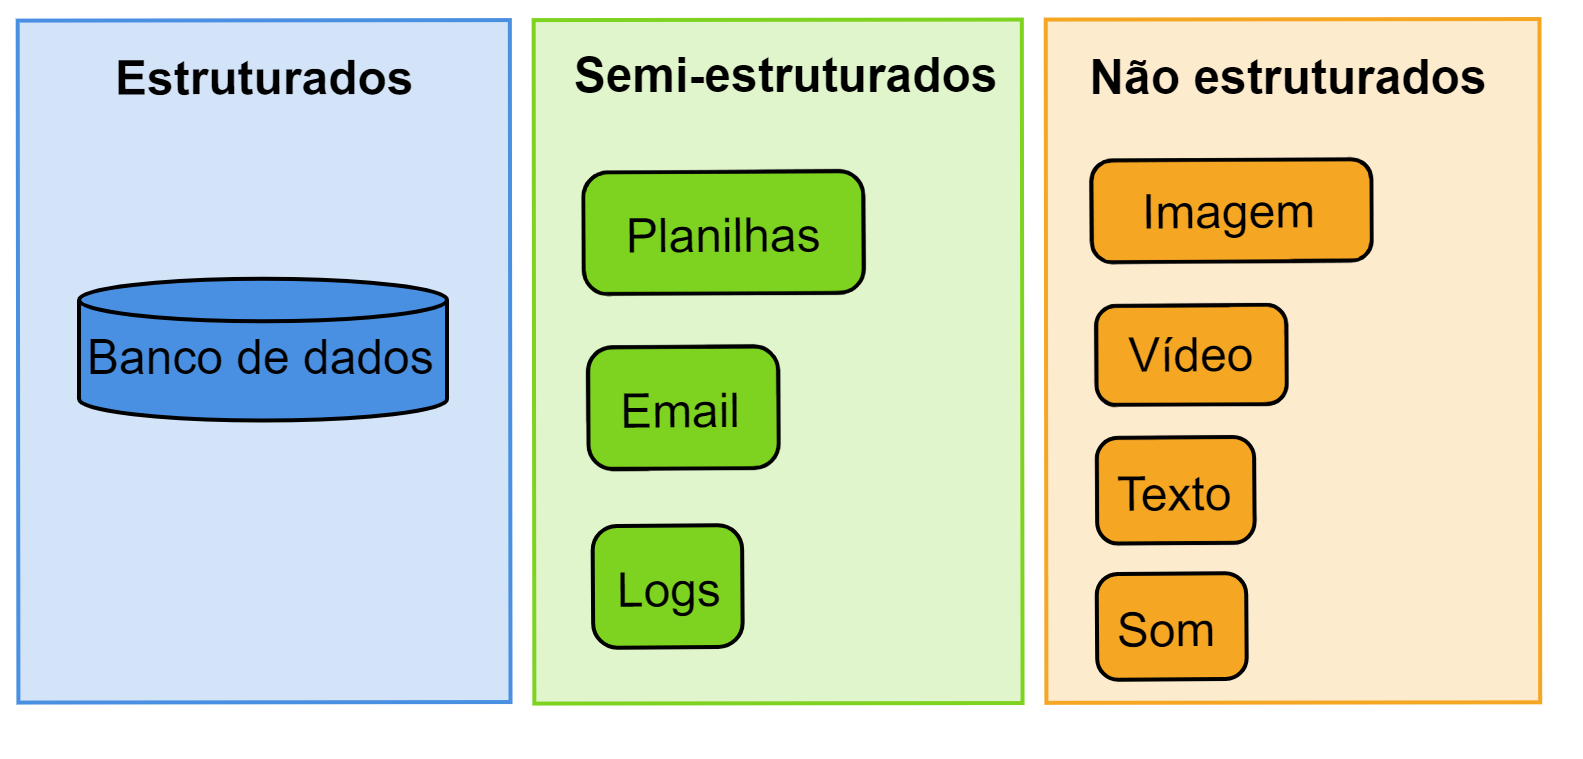
\includegraphics[scale=0.2]{Figuras/naturezadata.png}
\end{figure}


\end{ftst}

%=====

\begin{ftst}{Originalidade}{Caracterização dos dados}
\vone
\begin{itemize}
    \item \textbf{Primários:} dados originais sem nenhum processamento.
    \vone
    \item \textbf{Secundários:} dados processados, agregados ou transformados.
    \vone
    \item \textbf{Terciário:} resultado de análises sobre os dados. Ex: gráficos e tabelas resumidas.
\end{itemize}
\end{ftst}

%=====

\begin{ftst}{Volume dos dados}{Caracterização dos dados}
\vone
\begin{itemize}
    \item \textbf{Small data:} cabem integralmente na memória (HD) de uma máquina comum.
    \vone
    \item \textbf{Big data:} 
    \begin{itemize}
        \item não cabem integralmente na memória. 
        \item necessidade de processamento distribuído.
        \item Além do volume, o big data também tem as características de Variedade e Velocidade.
    \end{itemize}

\end{itemize}
\end{ftst}

%=====

\begin{ftst}{Geração dos dados}{Caracterização dos dados}
\vone
\begin{itemize}
    \item \textbf{Naturais:} 
    \begin{itemize}
        \item \textbf{Observacionais:} coleta de dados sem intervenção no processo observado.
        \item \textbf{Intervencionais:} resultados de experimentos com intervenções nos valores.
    \end{itemize}
    \vone
    \item \textbf{Sintéticos:} dados gerados por um algoritmo ou um modelo generativo.

\end{itemize}
\end{ftst}

%=====

\begin{ftst}{Caracterização dos dados}{Introdução}

Os conjuntos de dados são formados por \textbf{objetos}, que por sua vez possuem\textbf{ atributos}.
\vone
\vone
\begin{center}
    \textit{atributos = atributos de entradas = vetor de características\\ = atributos preditivos}
\end{center}

\vone
Cada \textbf{objeto} corresponde a uma ocorrência dos dados. 
\vone
Cada \textbf{atributo} está associado a uma propriedade do objeto.

\end{ftst}

%=====

\begin{ftst}{Caracterização dos dados}{Introdução}

Os conjuntos de dados são formados por \textbf{objetos}, que por sua vez possuem\textbf{ atributos}.
\vone
\vone
\begin{center}
    \textit{atributos = atributos de entradas = vetor de características\\ = atributos preditivos}
\end{center}

\vone
Cada \textbf{objeto} corresponde a uma ocorrência dos dados. 
\vone
Cada \textbf{atributo} está associado a uma propriedade do objeto.

\end{ftst}

%=====

\begin{ftst}{Caracterização dos dados}{Análise dos dados}
Exemplo de conjunto de dados de pacientes de um hospital:

\begin{figure}
    \centering
    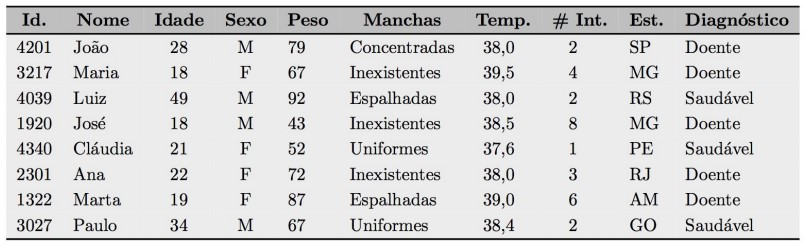
\includegraphics[scale=0.5]{Figuras/slide01_02.jpg}
\end{figure}

\scriptsize
- Cada linha representa 1 paciente.
\vone
- Cada paciente possui um vetor de características com Nome, Idade, Sexo, Peso, Manchas, Temperatura, Número de internações e Estado onde reside.
\vone
- Cada paciente também possui um atributo de saída (rótulo), que representa o fenômeno de interesse sobre o qual se deseja fazer previsões.
\vone
- Dependendo do problema, podem existir mais de um atributo de saída ou não existir nenhum.


\end{ftst}

%=====

\begin{ftst}{Caracterização dos dados}{Análise dos dados}
\small
Formalmente, os dados podem ser representados por uma matriz de objetos $X_n^d$, em que $n$ é o número de objetos e $d$ é o número de atributos de entrada.
\vone
O valor $d$ define a dimensionalidade dos objetos ou do espaço de objetos e podem ser vistos também como um conjunto de eixos ortogonais e os objetos, como pontos do espaço de dimensão $d$.
\vone
Já $n$ defini o volume da base de dados.

\begin{table}
	\begin{minipage}{0.4\linewidth}
		\centering
		\resizebox{\textwidth}{!}{%
		\begin{tabular}[width=\linewidth]{|c|l|c|}
		\centering
        \toprule
        \textbf{Exame 2} & \textbf{Exame 1} & \textbf{Diagnóstico} \\ 
        \midrule
        1 & 2 & Doente \\
    	1 & 10 & Saudável \\
    \bottomrule
    \end{tabular}}
	\end{minipage}\hfill
	\begin{minipage}{0.6\linewidth}
		\centering
		\label{figu:re}
		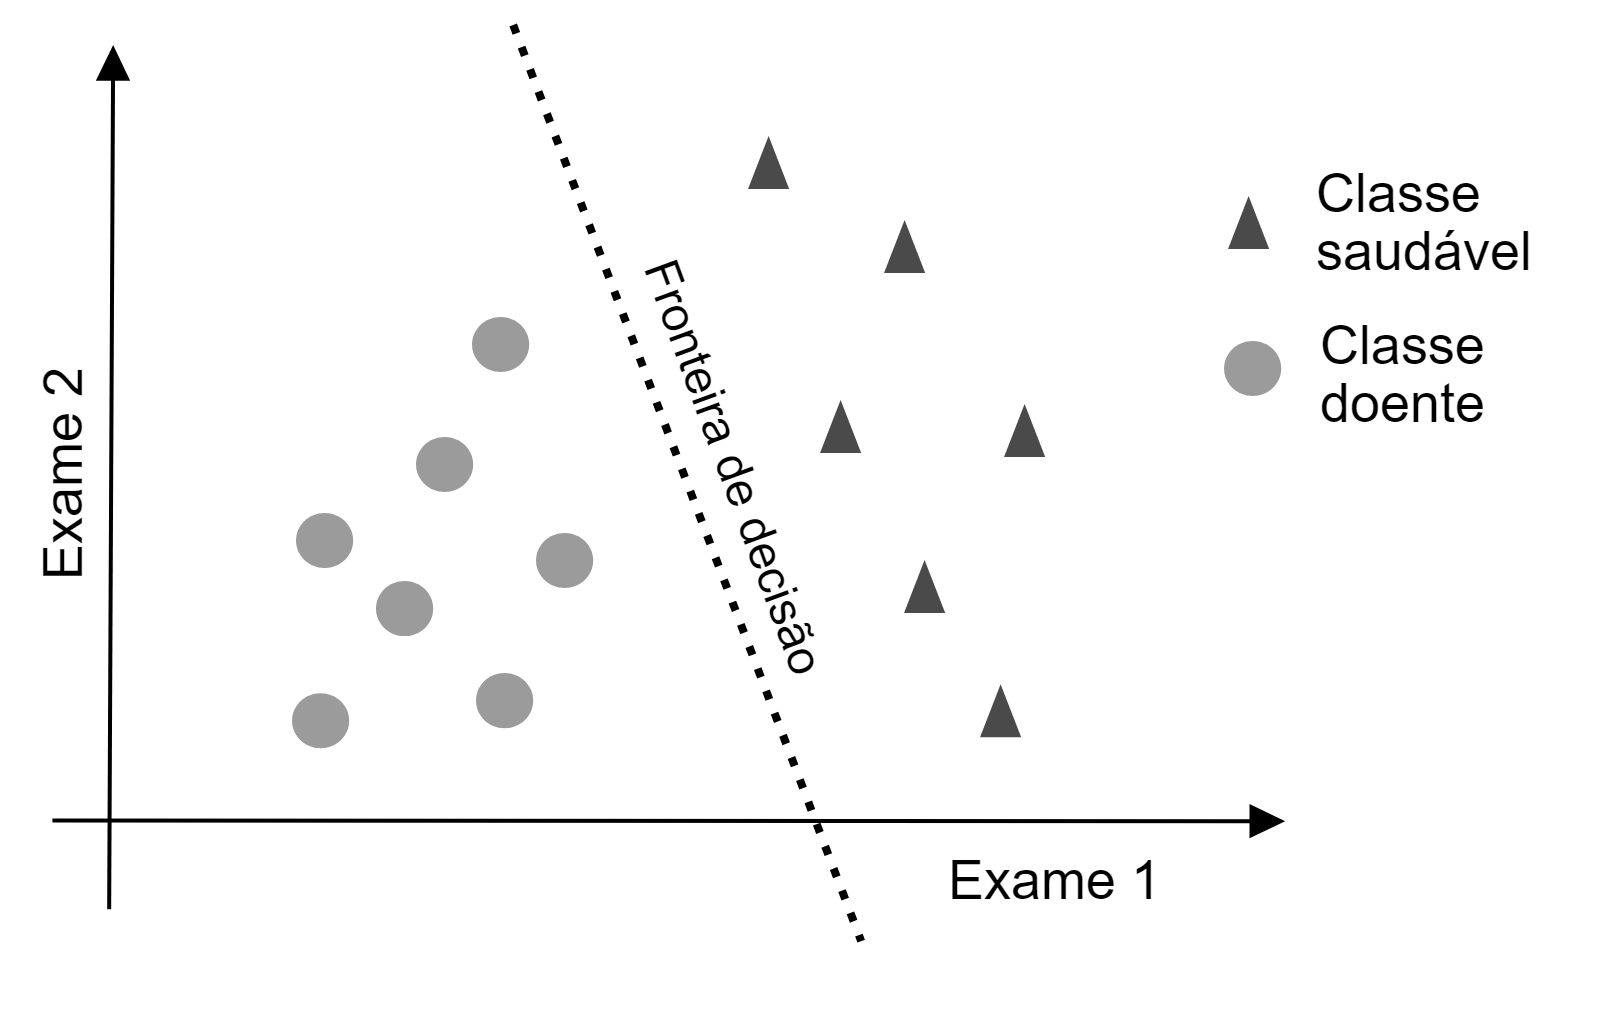
\includegraphics[width=0.8\textwidth]{Figuras/slide01_01.png}
	\end{minipage}
\end{table}


\end{ftst}

%=====


\begin{ftst}{Caracterização dos dados}{Análise dos dados}
Quando o atributo alvo contém rótulos que identificam categorias ou classes às quais os objetos pertencem, ele é denominado classe e assume valores discretos $1,...,k$.
\vone
\begin{center}
    \textit{Nesse caso temos um problema de classificação!}
\end{center}

\vone

\textbf{Classe majoritária:} classe que possui maior número de objetos.
\vone
\textbf{Classe minoritária: }classe que possui menor número de objetos.
\end{ftst}

%=====

\begin{ftst}{Caracterização dos dados}{Análise dos dados}
Se o atributo de saída contém valores numéricos contínuos, tem-se \textit{um problema de regressão!}
\vone
Uma caso especial de problema de regressão é a previsão de séries temporais.

\end{ftst}

%=====

\begin{ftst}{Caracterização dos dados}{Análise dos dados}
\textbf{Tipos de dados:} diz respeito ao grau de quantização nos dados.
\vone
\begin{itemize}
    \item Se o atributo representa quantidades, ele é denominado quantitativo ou numérico.\\
    \footnotesize
    \textit{Contínuo:} podem assumir um número infinito de valores.\\
    Exemplo: peso.\\
    \textit{Discreto:} assumem um número finito ou infinito contável.\\
    Exemplo: número de filhos.
    \vone
    \normalsize
    \item Se o atributo representa qualidade, ele é denominado qualitativo ou categórico.\\
    \footnotesize
    Exemplo: tamanho(baixa, média, alta) ou sexo(masculino, feminino).
\end{itemize}

\end{ftst}

%=====

\begin{ftst}{Caracterização dos dados}{Análise dos dados}
\textbf{Escala:} defini que operações podem ser realizadas sobre os valores.

\begin{itemize}
    \item Nominais: qualitativos e não possuem relação de ordem ($=$ e $\neq$).
    \item Ordinais: qualitativos e possuem relação de ordem ($=$, $\neq$, $<$, $>$, $\leq$ e $\geq$).
    \item Intervalares: quantitativos, representados por números dentro de um intervalo.
    \item Racionais: quantitativos e são os que mais carregam informações, pois seus valores têm significado absoluto.
\end{itemize}

\begin{figure}
    \centering
    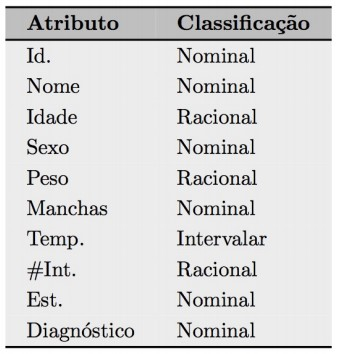
\includegraphics[scale=0.4]{Figuras/slide01_03.jpg}
\end{figure}



\end{ftst}

%=====

\begin{ftst}{Caracterização dos dados}{Análise dos dados}

\begin{itemize}
    \item \textbf{Completude:} 
    \begin{itemize}
        \item o quão representativos são os dados em relação ao fenômeno ou a população real?
        \item O volume de dados é suficiente?
    \end{itemize}
    \vone
    \item  \textbf{Integridade:} Os dados são coerentes?(falhas de coleta, transformações, armazenamento, etc.)
    \vone
    \item  \textbf{Atualidade:} quão recentes são os dados? Eles ainda são representativos?
\end{itemize}
\end{ftst}

%=====





\end{document}